%% Bản dịch tiếng Việt của elsarticle-template-num.tex (bản tiếng Anh là bản gốc để nộp).
%% Luôn cập nhật song song với bản tiếng Anh. Biên dịch bằng pdflatex như bản
%% tiếng Anh; cần gói vntex (Ubuntu: sudo apt install texlive-lang-other).
\documentclass[preprint,12pt]{elsarticle}

\usepackage[T5]{fontenc}
\usepackage[utf8]{inputenc}
\usepackage{amssymb}
\usepackage{amsmath}
\usepackage{booktabs}
\usepackage{graphicx}
\usepackage{float}
\usepackage{url}
\usepackage{array}
\usepackage{multirow}
\usepackage{adjustbox}
\usepackage{etoolbox}
\usepackage[section]{placeins}
\usepackage[hidelinks]{hyperref}
\usepackage[expansion=false]{microtype}
% Let lines with long hyphenated compounds stretch instead of overflowing.
\setlength{\emergencystretch}{2em}

% Keep floats in the section that cites them instead of drifting to the end.
\renewcommand{\topfraction}{0.9}
\renewcommand{\bottomfraction}{0.8}
\renewcommand{\textfraction}{0.07}
\renewcommand{\floatpagefraction}{0.75}
\setcounter{topnumber}{3}
\setcounter{totalnumber}{4}

% Table captions sit above the table: separate them from the top rule and
% give rows a little more vertical room.
\AtBeginEnvironment{table}{\setlength{\belowcaptionskip}{6pt}\renewcommand{\arraystretch}{1.15}}
\newcommand{\colhead}[1]{\begin{tabular}[b]{@{}c@{}}#1\end{tabular}}
\AtBeginEnvironment{table*}{\setlength{\belowcaptionskip}{6pt}\renewcommand{\arraystretch}{1.15}}

% Vietnamese captions and headings.
\abstracttitle{Tóm tắt}
\keywordtitle{Từ khóa}
\renewcommand{\figurename}{Hình}
\renewcommand{\tablename}{Bảng}
\renewcommand{\refname}{Tài liệu tham khảo}

\journal{Biomedical Signal Processing and Control}

\begin{document}

\begin{frontmatter}

\title{Học không gian trạng thái chọn lọc thích ứng miền cho giải mã EEG tưởng tượng vận động liên chủ thể}

\author[aff1]{[Tên] [Họ]\corref{cor1}}
\ead{dinhmanhcuong2003@gmail.com}
\cortext[cor1]{Tác giả liên hệ.}

\affiliation[aff1]{organization={[Khoa], [Tên đầy đủ của cơ quan]},
                   addressline={[Địa chỉ]},
                   city={[Thành phố]},
                   postcode={[Mã bưu chính]},
                   country={[Quốc gia]}}

\begin{abstract}
Giải mã điện não đồ tưởng tượng vận động (MI-EEG) liên chủ thể gặp khó khăn do tỉ số tín hiệu trên nhiễu thấp, dữ liệu có nhãn khan hiếm, và độ dịch chuyển phân phối lớn giữa các chủ thể và các phiên ghi. Nghiên cứu này đề xuất SSM-DAN, một mạng không gian trạng thái chọn lọc thích ứng miền, kết hợp khối tích chập đa thang với các khối không gian trạng thái chọn lọc hai chiều để nắm bắt cả mẫu thời gian cục bộ lẫn tầm xa, đồng thời giảm độ dịch chuyển giữa các chủ thể bằng căn chỉnh phân cấp, gồm một lớp chuẩn hóa nguồn--đích được học và thích ứng tại thời điểm kiểm thử không cần nhãn. Khung phương pháp được đánh giá trên ba bộ dữ liệu MI-EEG công khai theo giao thức kiểm định bỏ-một-chủ-thể (leave-one-subject-out) với các phiên huấn luyện, thích ứng và kiểm thử được tách theo thứ tự thời gian. SSM-DAN đạt độ chính xác trung bình 76,12\% trên BCI Competition IV-2a, 84,09\% trên BCI Competition IV-2b và 84,33\% trên Zhou2016. Các nghiên cứu loại bỏ thành phần (ablation) cho thấy đóng góp của từng thành phần thích ứng phụ thuộc vào bộ dữ liệu. Kết quả cho thấy việc kết hợp mô hình không gian trạng thái chọn lọc với căn chỉnh phân cấp được học giúp cải thiện giải mã MI liên chủ thể mà không cần nhãn của chủ thể đích.
\end{abstract}

\begin{keyword}
tưởng tượng vận động \sep điện não đồ \sep giao diện não--máy tính \sep mô hình không gian trạng thái chọn lọc \sep Mamba \sep thích ứng miền \sep thích ứng tại thời điểm kiểm thử
\end{keyword}

\end{frontmatter}

\section{Giới thiệu}
\label{sec:introduction}

Giao diện não--máy tính dựa trên tưởng tượng vận động (MI-BCI) giải mã ý định vận động từ điện não đồ (EEG) không xâm lấn, phục vụ phục hồi chức năng, giao tiếp và điều khiển. Các mẫu mất đồng bộ và đồng bộ liên quan đến sự kiện mà MI-BCI dựa vào thường yếu, không dừng, và khác nhau giữa các chủ thể cũng như giữa các phiên ghi của cùng một chủ thể \cite{pfurtscheller1999erd}. Vì vậy, một bộ giải mã huấn luyện trên những người dùng có sẵn thường suy giảm hiệu năng trên người dùng mới, trong khi việc hiệu chuẩn từng người dùng mới bằng các lần thử có nhãn vừa tốn thời gian vừa gây mệt mỏi \cite{lotte2015signal}. Giảm hoặc loại bỏ bước hiệu chuẩn có nhãn này do đó là một yêu cầu cốt lõi để MI-BCI có thể dùng trong thực tế.

Các bộ giải mã MI ban đầu đi theo quy trình học máy cổ điển. Lọc mẫu không gian chung (CSP) \cite{ramoser2000optimal} và phiên bản dải lọc FBCSP \cite{ang2012filterbank}, phương pháp thắng cuộc thi BCI Competition~IV, trích xuất đặc trưng công suất dải tần qua các bước thiết kế thủ công, riêng cho từng chủ thể, rồi đưa vào một bộ phân loại tuyến tính. Về sau, học sâu thay thế các bước này bằng học đặc trưng đầu--cuối: ShallowConvNet và DeepConvNet \cite{schirrmeister2017deep} cùng mạng gọn nhẹ EEGNet \cite{lawhern2018eegnet} học trực tiếp các bộ lọc phổ và không gian từ EEG thô. Các mô hình sau đó mở rộng ngữ cảnh thời gian: EEG Conformer thêm cơ chế tự chú ý vào khối tích chập \cite{song2023eegconformer}, ATCNet kết hợp chú ý với mạng tích chập thời gian (TCN) giãn \cite{altaheri2023atcnet}, và TCFormer ghép tích chập đa thang, Transformer và TCN \cite{altaheri2025tcformer}. Tuy nhiên, tự chú ý có chi phí bậc hai theo độ dài chuỗi \cite{vaswani2017attention} và cần nhiều dữ liệu hơn mức các bộ EEG thường có. Gần đây, các mô hình không gian trạng thái (SSM), từ S4 có cấu trúc \cite{gu2022s4} đến Mamba chọn lọc \cite{gu2024mamba}, nổi lên như một lựa chọn thay thế có chi phí tăng tuyến tính theo độ dài chuỗi; trong mô hình hóa ngôn ngữ, Mamba đạt hoặc vượt Transformer có kích thước tương đương, đồng thời cho thông lượng sinh cao hơn nhiều lần \cite{gu2024mamba}. Sau đó, MI-Mamba và một mạng Mamba không gian--thời gian đã kết hợp SSM với tích chập để giải mã MI \cite{guo2025mimamba,yang2025stmamba}. Tất cả các bộ giải mã kể trên, từ CSP đến Mamba, chỉ học từ các chủ thể nguồn, nên độ chính xác trên chủ thể mới phụ thuộc vào mức độ tương đồng với các chủ thể này.

Một hướng nghiên cứu bổ sung nhằm giảm sự phụ thuộc này vào tập huấn luyện và vào việc hiệu chuẩn có nhãn cho từng người dùng. Các mô hình nền tảng (foundation model) cho EEG, được tiền huấn luyện trên kho dữ liệu lớn và đa dạng, chẳng hạn khoảng 2.500 giờ EEG của LaBraM \cite{jiang2024labram,wang2024eegpt}, là một hướng nhiều tiềm năng, nhưng đòi hỏi thu thập và chuẩn hóa các bộ dữ liệu lớn, không đồng nhất, và thường vẫn cần tinh chỉnh bằng dữ liệu có nhãn của tác vụ đích. Chuyển giao giữa các chủ thể trong cùng một tác vụ là một lựa chọn nhẹ hơn. Tổng quát hóa miền học từ nhiều chủ thể nguồn các đặc trưng có thể dùng cho chủ thể chưa thấy, nhờ đó người dùng mới có thể sử dụng ngay mà không cần hiệu chuẩn \cite{liu2023stdg,zhong2025eegdg,zheng2025crosssubject}; tuy nhiên, do chủ thể đích không bao giờ được quan sát, độ dịch chuyển riêng của chủ thể đó không thể được bù trừ. Thích ứng miền khắc phục hạn chế này bằng cách sử dụng thêm EEG không nhãn của chủ thể mới. Dữ liệu này không cần gán nhãn cho bất kỳ lần thử nào, nên bộ giải mã được điều chỉnh theo từng người dùng mà vẫn tránh được phiên hiệu chuẩn có nhãn.

Trong thích ứng miền không giám sát (UDA), căn chỉnh Riemann (RA) và căn chỉnh Euclid giảm dịch chuyển ở mức đầu vào bằng cách làm trắng các lần thử của mỗi chủ thể theo hiệp phương sai trung bình của chủ thể đó \cite{zanini2018riemannian,he2020euclidean}. Ở mức đặc trưng, độ sai khác trung bình cực đại (MMD), được DAN đưa vào mạng sâu dưới dạng đa nhân \cite{long2015dan}, là một trong những tiêu chí căn chỉnh được sử dụng rộng rãi nhất trong các phương pháp thích ứng miền nhờ tính phi tham số và tối ưu ổn định, và cũng được dùng trong các mô hình EEG như RMETNet \cite{zhao2026rmetnet}. Huấn luyện đối kháng với bộ phân biệt miền \cite{ganin2016dann,tang2020cdan} và căn chỉnh dựa trên nguyên mẫu lớp \cite{zhang2024prototypeda} cung cấp các mục tiêu bổ trợ. Việc căn chỉnh miền cũng có thể được thực hiện bên trong mạng thông qua các lớp chuẩn hóa: trong thích ứng miền thị giác, AutoDIAL \cite{carlucci2017autodial} đề xuất các lớp căn chỉnh miền học mức độ trộn giữa thống kê nguồn và đích khi chuẩn hóa. Ý tưởng này là nguồn cảm hứng cho cơ chế chuẩn hóa ở mức đặc trưng trong nghiên cứu này.

Ngoài ra, độ chính xác liên chủ thể được báo cáo thường khó so sánh, do một số giao thức kiểm thử trong cùng phiên, chọn epoch bằng nhãn đích, hoặc thích ứng trên chính các lần thử đánh giá \cite{miao2025satransnet,zhao2026rmetnet,liao2025eegencoder} (Mục~\ref{subsec:published}). Vì vậy, chúng tôi đề xuất SSM-DAN, một mạng không gian trạng thái chọn lọc hai chiều với thích ứng phân cấp không cần nhãn, và đánh giá theo giao thức theo thời gian, giữ nhãn đích nằm ngoài huấn luyện, thích ứng và chọn mô hình \cite{jayaram2018moabb}. Các đóng góp gồm:
\begin{itemize}
    \item một bộ giải mã đầu--cuối kết hợp tích chập đa thang, các khối không gian trạng thái chọn lọc quét xuôi/ngược xen kẽ, và hợp nhất cục bộ--toàn cục bằng TCN;
    \item một chiến lược thích ứng phân cấp giảm độ dịch chuyển giữa các chủ thể ở mức đầu vào, đặc trưng và dự đoán mà không cần nhãn đích, bao gồm một lớp chuẩn hóa nguồn--đích được học lấy cảm hứng từ AutoDIAL; và
    \item một giao thức đánh giá bỏ-một-chủ-thể nghiêm ngặt theo thứ tự thời gian trên ba bộ dữ liệu MI-EEG công khai, trong đó mọi phương pháp cơ sở được huấn luyện lại trong cùng điều kiện, với độ chính xác theo từng chủ thể, hệ số $\kappa$ của Cohen, kiểm định thống kê, phân tích hiệu năng tính toán và loại bỏ từng thành phần.
\end{itemize}

\section{Phương pháp}
\label{sec:method}

\begin{figure*}[!htbp]
    \centering
    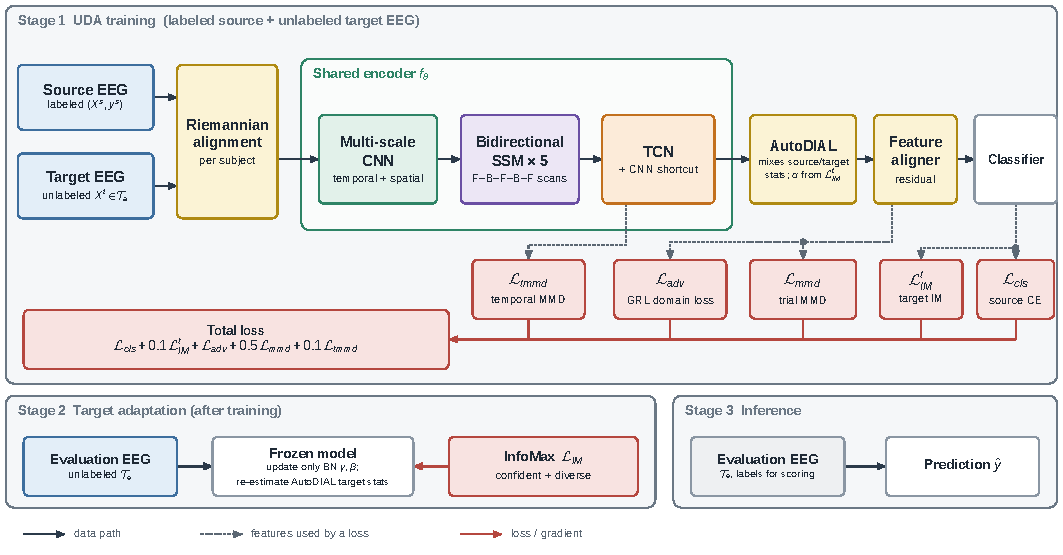
\includegraphics[width=\textwidth]{figures/architecture_overview.pdf}
    \caption{Tổng quan SSM-DAN: huấn luyện với EEG nguồn có nhãn và EEG đích không nhãn (Giai đoạn~1), thích ứng tại thời điểm kiểm thử không cần nhãn trên các phiên đánh giá không nhãn $\mathcal{T}_e$ (Giai đoạn~2), và dự đoán (Giai đoạn~3).}
    \label{fig:architecture_overview}
\end{figure*}

SSM-DAN gồm hai phần (Hình~\ref{fig:architecture_overview}). Bộ mã hóa EEG kết hợp tích chập đa thang cho đặc trưng phổ--không gian cục bộ, các khối không gian trạng thái chọn lọc hai chiều cho động học tầm xa, và một đầu hợp nhất tích chập thời gian (Mục~\ref{subsec:conv_frontend}--\ref{subsec:tcn}). Lược đồ thích ứng phân cấp giảm độ dịch chuyển giữa các chủ thể ở ba mức: làm trắng Riemann cho đầu vào, chuẩn hóa AutoDIAL kèm hàm mất mát đối kháng và sai khác phân phối cho đặc trưng, và thích ứng tại thời điểm kiểm thử cho dự đoán (Mục~\ref{subsec:ra}--\ref{subsec:imtta}). Mô hình được huấn luyện trên các lần thử có nhãn của chủ thể nguồn và các lần thử không nhãn của chủ thể đích (Giai đoạn~1), được thích ứng với các lần thử đánh giá không nhãn (Giai đoạn~2), rồi dùng để dự đoán (Giai đoạn~3).

\subsection{Bộ mã hóa tích chập đa thang}
\label{subsec:conv_frontend}

Mỗi lần thử $X\in\mathbb{R}^{C\times T}$ ($C$ điện cực, $T$ mẫu) đi qua ba tích chập thời gian với kích thước nhân 20, 32 và 64 mẫu như trong TCFormer \cite{altaheri2025tcformer}, tiếp theo là lọc không gian theo chiều sâu (depthwise), gộp (pooling), và tinh chỉnh theo nhóm xuống 16 kênh cho mỗi thang. Một cơ chế chú ý nhóm kênh có kết nối tắt gán một trọng số sigmoid cho mỗi thang, và bước gộp thứ hai tạo ra chuỗi đặc trưng cục bộ $H_c\in\mathbb{R}^{48\times L}$.

\subsection{Bộ mã hóa không gian trạng thái chọn lọc hai chiều}
\label{subsec:ssm}

\begin{figure}[H]
    \centering
    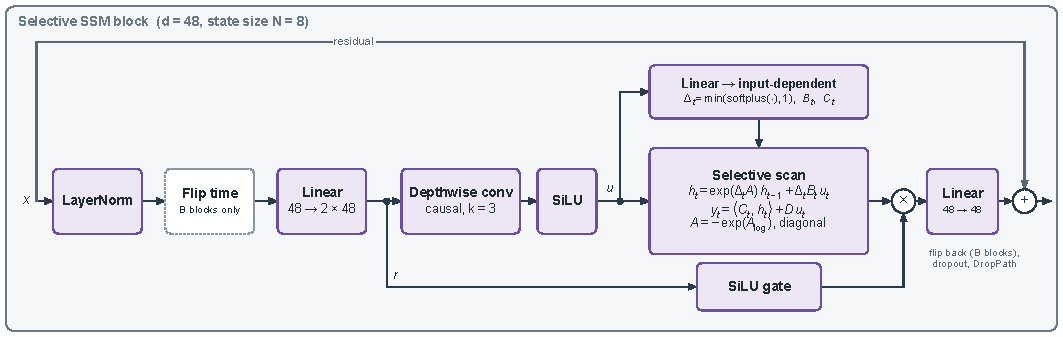
\includegraphics[width=\textwidth]{figures/ssm_block.pdf}
    \caption{Khối SSM chọn lọc. Khối quét ngược đảo và khôi phục trục thời gian quanh bộ trộn; khối quét xuôi bỏ qua các thao tác này.}
    \label{fig:ssm_block}
\end{figure}

Để nắm bắt các phụ thuộc trên toàn bộ lần thử, $H_c$ đi qua năm khối không gian trạng thái chọn lọc \cite{gu2022s4,gu2024mamba}, mỗi khối điều khiển một phép hồi quy đường chéo với đầu vào đã chiếu $u_t$:
\begin{align}
    h_t &= \exp(\Delta_t A)\odot h_{t-1} + \Delta_t B_t\odot u_t, \\
    z_t &= C_t^\top h_t + d\odot u_t ,
\end{align}
trong đó $A=-\exp(A_{\log})$ là hệ số suy giảm ổn định được học, còn $\Delta_t$, $B_t$ và $C_t$ phụ thuộc vào đầu vào, nhờ đó mỗi khối chọn bước thời gian cần giữ lại với chi phí tuyến tính. Các khối xen kẽ quét xuôi và quét ngược (Hình~\ref{fig:ssm_block}), cho ngữ cảnh hai chiều mà không cần thêm khối. Số chiều trạng thái là tám, với dropout 0,4 và độ sâu ngẫu nhiên (stochastic depth).

\subsection{Hợp nhất cục bộ--toàn cục và phân loại}
\label{subsec:tcn}

Đầu ra không gian trạng thái được giảm xuống 16 kênh và ghép với chuỗi cục bộ 48 kênh $H_c$, để đầu phân loại thấy được cả bằng chứng cục bộ lẫn toàn cục. Hai khối mạng tích chập thời gian (TCN) theo nhóm có kết nối tắt, với độ dài nhân bốn và hệ số giãn một và hai, tinh chỉnh chuỗi 64 kênh thu được. Trung bình của bước thời gian cuối và giá trị trung bình theo thời gian tạo thành biểu diễn lần thử $q\in\mathbb{R}^{64}$, gồm bốn nhóm 16 kênh (ba thang tích chập và nhánh không gian trạng thái). Một bộ phân loại theo nhóm có ràng buộc chuẩn tạo một tập điểm lớp cho mỗi nhóm, rồi kết hợp bằng các trọng số softmax được học.

\subsection{Căn chỉnh tín hiệu Riemann}
\label{subsec:ra}

Do cấu trúc hiệp phương sai EEG bị dịch chuyển giữa các chủ thể, căn chỉnh Riemann (RA) làm trắng các lần thử của mỗi chủ thể bằng căn bậc hai nghịch đảo của hiệp phương sai trung bình $\bar{R}$ của chủ thể đó, tức trung bình Riemann bất biến afin của các hiệp phương sai lần thử đã co rút OAS \cite{zanini2018riemannian,he2020euclidean}:
\begin{equation}
    \widetilde{X}=\bar{R}^{-1/2}X.
\end{equation}
Để tránh rò rỉ thông tin, $\bar{R}$ chỉ được ước lượng từ dữ liệu có sẵn trước khi đánh giá rồi áp dụng không đổi: từ các phiên huấn luyện cho các phiên kiểm định của mỗi chủ thể nguồn, và từ các phiên trước không nhãn $\mathcal{T}_a$ cho các phiên đánh giá $\mathcal{T}_e$ của chủ thể đích.

\subsection{Lớp căn chỉnh miền tự động}
\label{subsec:autodial}

Làm trắng Riemann căn chỉnh thống kê đầu vào nhưng không xử lý được các dịch chuyển phát sinh bên trong mạng. Vì vậy, theo AutoDIAL \cite{carlucci2017autodial}, biểu diễn lần thử $q$ được chuẩn hóa bằng một lớp học mức độ chuẩn hóa đặc trưng đích bằng thống kê của chính nó: đặc trưng nguồn dùng mô-men nguồn $(\mu_s,\sigma_s^2)$, còn đặc trưng đích dùng mô-men của hỗn hợp giữa phân phối nguồn và phân phối đích $(\mu_t,\sigma_t^2)$,
\begin{align}
    \mu_\alpha &= \alpha\mu_t+(1-\alpha)\mu_s, \\
    \sigma_\alpha^2 &= \alpha\sigma_t^2+(1-\alpha)\sigma_s^2+\alpha(1-\alpha)(\mu_t-\mu_s)^2,
\end{align}
sao cho
\begin{equation}
    \hat{q}^s = \gamma\odot\frac{q^s-\mu_s}{\sqrt{\sigma_s^2+\epsilon}}+\beta, \qquad
    \hat{q}^t = \gamma\odot\frac{q^t-\mu_\alpha}{\sqrt{\sigma_\alpha^2+\epsilon}}+\beta ,
\end{equation}
với các tham số afin dùng chung $\gamma$ và $\beta$. Trọng số trộn $\alpha\in(0,1)$, khởi tạo bằng 0,5 và được học riêng cho từng nhóm trong bốn nhóm đặc trưng, nội suy giữa thống kê nguồn ($\alpha\rightarrow0$) và thống kê đích ($\alpha\rightarrow1$). Các mô-men được tính theo từng mini-batch khi huấn luyện và được theo dõi bằng trung bình trượt (momentum 0,1), rồi được trộn với $\alpha$ đã học khi suy luận; các lần thử kiểm định nguồn luôn dùng thống kê nguồn.

\subsection{Hàm mục tiêu huấn luyện}
\label{subsec:uda}

Một bộ căn chỉnh có kết nối tắt $64\!\rightarrow\!128\!\rightarrow\!64$ đặt trước bộ phân loại và các hàm mất mát căn chỉnh. Ngoài hàm entropy chéo trên dữ liệu nguồn $\mathcal{L}_{\mathrm{cls}}$, Giai đoạn~1 dùng hàm mất mát miền với lớp đảo gradient $\mathcal{L}_{\mathrm{adv}}$ \cite{ganin2016dann}, các hàm MK-MMD trên biểu diễn lần thử ($\mathcal{L}_{\mathrm{mmd}}$) và trên chuỗi TCN ($\mathcal{L}_{\mathrm{tmmd}}$) \cite{long2015dan}, và hàm cực đại hóa thông tin \cite{liang2020shot}
\begin{equation}
    \mathcal{L}_{\mathrm{IM}}
    =\frac{1}{N}\sum_{j=1}^{N} H(p_j)-H\!\left(\frac{1}{N}\sum_{j=1}^{N}p_j\right),
\label{eq:im}
\end{equation}
trong đó $p_j$ là phân phối lớp dự đoán của lần thử thứ $j$ trong $N$ lần thử không nhãn và $H(\cdot)$ là entropy. Hàm mục tiêu là
\begin{equation}
    \mathcal{L}=\mathcal{L}_{\mathrm{cls}}+0.1\mathcal{L}_{\mathrm{IM}}^{t}+\mathcal{L}_{\mathrm{adv}}
    +0.5\mathcal{L}_{\mathrm{mmd}}+0.1\mathcal{L}_{\mathrm{tmmd}}.
\label{eq:total_loss}
\end{equation}
trong đó $\mathcal{L}_{\mathrm{IM}}^{t}$ được tính trên các lần thử đích thuộc $\mathcal{T}_a$. Các hàm mất mát căn chỉnh nhận đầu ra AutoDIAL với $\alpha$ cố định, nên $\alpha$ chỉ được học qua $\mathcal{L}_{\mathrm{IM}}^{t}$.

\subsection{Thích ứng tại thời điểm kiểm thử}
\label{subsec:imtta}

Checkpoint có độ chính xác kiểm định nguồn cao nhất được thích ứng với các lần thử đánh giá không nhãn $\mathcal{T}_e$ bằng thích ứng tại thời điểm kiểm thử dựa trên cực đại hóa thông tin (IM-TTA): chỉ các hệ số tỉ lệ và độ dời của BatchNorm được cập nhật, giúp hạn chế quá khớp với tập đích nhỏ \cite{wang2021tent}, bằng cách cực tiểu hóa Pt.~\eqref{eq:im} trên $\mathcal{T}_e$ trong năm lượt Adam (tốc độ học $10^{-4}$). Sau đó, các mô-men đích của AutoDIAL được ước lượng lại trong một lượt trên cùng các lần thử đó, với $\alpha$ và mô-men nguồn cố định. Nhãn của $\mathcal{T}_e$ chỉ được dùng để chấm điểm.

\section{Thiết lập thực nghiệm}
\label{sec:experiments}

\subsection{Bộ dữ liệu}
\label{sec:datasets}

Ba bộ dữ liệu MI-EEG công khai, truy cập qua MOABB/Braindecode \cite{jayaram2018moabb}, được sử dụng (Bảng~\ref{tab:datasets}).

\begin{table*}[!htbp]
\centering
\caption{Tóm tắt các bộ dữ liệu MI-EEG (không tính kênh EOG).}
\label{tab:datasets}
\small
\setlength{\tabcolsep}{4.5pt}
\begin{tabular}{lcccl}
\toprule
Bộ dữ liệu & Số chủ thể & Số kênh & Số phiên & Các lớp \\
\midrule
BCI IV-2a & 9 & 22 & 2 & tay trái, tay phải, chân, lưỡi \\
BCI IV-2b & 9 & 3  & 5 & tay trái, tay phải \\
Zhou2016  & 4 & 14 & 3 & tay trái, tay phải, chân \\
\bottomrule
\end{tabular}
\end{table*}

\subsubsection{BCI Competition IV-2a}
\label{subsec:bcic2a}

Chín người tham gia được ghi trong hai phiên vào các ngày khác nhau, mỗi phiên gồm 288 lần thử tưởng tượng tay trái, tay phải, hai chân và lưỡi, từ 22 điện cực EEG ở tần số 250~Hz (lọc thông dải 0,5--100~Hz, lọc chặn 50~Hz; ba kênh EOG không được sử dụng) \cite{tangermann2012review}.

\subsubsection{BCI Competition IV-2b}
\label{subsec:bcic2b}

Chín người tham gia thuận tay phải, lấy từ một nghiên cứu gồm mười người ($24,7\pm3,3$ tuổi) \cite{leeb2007virtual}, thực hiện tưởng tượng tay trái so với tay phải, được ghi từ ba đạo trình lưỡng cực quanh C3, Cz và C4 ở 250~Hz (ba kênh EOG không được sử dụng). Các phiên 1--3 là phần hiệu chuẩn và các phiên 4--5 là phần đánh giá \cite{tangermann2012review}; cách chia theo thời gian này được giữ nguyên, và bộ dữ liệu kiểm tra xem phương pháp còn hữu ích hay không khi chỉ có ba điện cực.

\subsubsection{Zhou2016}
\label{subsec:zhou2016}

Bốn người tham gia khỏe mạnh (22--28 tuổi), mỗi người được ghi trong ba phiên cách nhau từ vài ngày đến vài tháng \cite{zhou2016trialselection}. Mỗi phiên có hai lượt ghi gồm 75 lần thử (25 lần mỗi lớp: tay trái, tay phải, chân) từ 14 điện cực ở 250~Hz; mỗi lần thử gồm 5~s gợi ý tưởng tượng, sau đó 4~s nghỉ.

\subsection{Giao thức LOSO theo thời gian có thích ứng tại thời điểm kiểm thử}
\label{subsec:clean_protocol}

Mỗi lượt bỏ-một-chủ-thể (LOSO) giữ lại một chủ thể đích và dùng các chủ thể còn lại làm nguồn có nhãn, với cách chia phiên trong Bảng~\ref{tab:protocol}. Các phiên trước của chủ thể đích được dùng không kèm nhãn ở Giai đoạn~1; các phiên đánh giá bị loại khỏi huấn luyện và chọn mô hình, và EEG không nhãn của chúng chỉ được IM-TTA dùng trước khi chấm điểm.

\begin{table*}[!htbp]
\centering
\caption{Phân bổ phiên theo thời gian trong mỗi lượt LOSO. Nhãn của phiên đánh giá chỉ được dùng để chấm điểm.}
\label{tab:protocol}
\small
\setlength{\tabcolsep}{5pt}
\begin{tabular}{lcccc}
\toprule
\multirow{2}{*}{Bộ dữ liệu} & \multicolumn{2}{c}{Chủ thể nguồn (có nhãn)} & \multicolumn{2}{c}{Chủ thể đích} \\
\cmidrule(lr){2-3}\cmidrule(lr){4-5}
 & Huấn luyện & Kiểm định & \colhead{UDA Giai đoạn~1\\(không nhãn)} & \colhead{IM-TTA + đánh giá\\(ẩn nhãn)} \\
\midrule
BCI IV-2a & phiên 1      & phiên 2      & phiên 1      & phiên 2 \\
BCI IV-2b & phiên 1--3  & phiên 4--5  & phiên 1--3  & phiên 4--5 \\
Zhou2016  & phiên 1--2  & phiên 3      & phiên 1--2  & phiên 3 \\
\bottomrule
\end{tabular}
\end{table*}

Như vậy có chín lượt cho BCI IV-2a và IV-2b, bốn lượt cho Zhou2016, với siêu tham số giống nhau ở mọi lượt; checkpoint có độ chính xác kiểm định nguồn cao nhất được sử dụng. Với Zhou2016, điểm đích trên tất cả các phiên được báo cáo như một chỉ số chẩn đoán phụ.


\subsection{Tiền xử lý và tăng cường dữ liệu}
\label{subsec:preprocessing}

Các kênh EEG được lấy mẫu lại về 250~Hz và đổi sang microvolt. BCI IV-2a dùng toàn bộ cửa sổ sự kiện của MOABB và BCI IV-2b bỏ 0,5~s cuối, cả hai không lọc; Zhou2016 được lọc thông dải 8--30~Hz và cắt đoạn 0,5--5,0~s sau khi xuất hiện gợi ý.

Thống kê chuẩn hóa z-score được khớp trên phần huấn luyện nguồn. Với BCI IV-2a và IV-2b, các mini-batch nguồn có nhãn được nhân đôi bằng phép tăng cường phân đoạn và tái tổ hợp (S\&R) \cite{lotte2015signal} mà TCFormer sử dụng \cite{altaheri2025tcformer}, ghép lại các mảnh tám đoạn từ các lần thử cùng lớp; Zhou2016 không dùng tăng cường.

\subsection{Chi tiết cài đặt}
\label{subsec:training}

Mọi thí nghiệm chạy trên Kaggle notebook với một GPU NVIDIA Tesla T4 (16~GB). BCI IV-2a và IV-2b dùng kích thước batch 48, tối đa 125 epoch, và Adam (tốc độ học $9\times10^{-4}$, $\beta_1=0,5$, suy giảm trọng số $10^{-3}$); Zhou2016 dùng kích thước batch 32, 100 epoch, tốc độ học $10^{-3}$ và suy giảm trọng số $10^{-4}$. Ba epoch khởi động tuyến tính được theo sau bởi suy giảm cosin. Hạt giống ngẫu nhiên (0), cách chia dữ liệu và khởi tạo là chung cho mọi phương pháp và biến thể, nên mỗi phép so sánh chỉ khác nhau ở thành phần được đánh giá.

\subsection{Các phương pháp so sánh}
\label{subsec:baselines}

Các phương pháp cơ sở được nhóm theo mức truy cập dữ liệu đích: chỉ dùng nguồn gồm EEG Conformer \cite{song2023eegconformer}, ATCNet \cite{altaheri2023atcnet}, TCFormer \cite{altaheri2025tcformer}, EEGEncoder \cite{liao2025eegencoder} và SATrans-Net \cite{miao2025satransnet}; dựa trên UDA là RMETNet \cite{zhao2026rmetnet}; và thích ứng tại thời điểm kiểm thử gồm T-TIME \cite{li2024ttime} và BFT \cite{li2026bft}. Mỗi phương pháp được so sánh với biến thể SSM-DAN có cùng mức truy cập dữ liệu đích. Tất cả các phương pháp được huấn luyện lại từ mã nguồn công bố với cùng các lượt LOSO, cách chia theo thời gian, tiền xử lý, hạt giống ngẫu nhiên và cách chọn checkpoint chỉ dựa trên nguồn; nhãn đánh giá không bao giờ tham gia huấn luyện hay chọn mô hình. Tối ưu hóa riêng của từng mô hình theo khuyến nghị gốc. Kết quả công bố theo các giao thức khác được báo cáo riêng ở Mục~\ref{subsec:published}. Để ổn định số, hiệp phương sai của RMETNet trên Zhou2016 được cộng thêm một hệ số ridge bằng $10^{-3}$ lần trị riêng trung bình.

\subsection{Thước đo đánh giá và cách báo cáo}
\label{subsec:metrics}

Độ chính xác và $\kappa$ của Cohen được báo cáo dưới dạng trung bình $\pm$ độ lệch chuẩn trên các chủ thể đích. Tốc độ truyền thông tin (ITR) \cite{wolpaw2002bci} biểu diễn độ chính xác $P$ trên $N$ lớp là
\begin{equation}
\mathrm{ITR}=\frac{60}{T}\left[\log_2 N+P\log_2 P+(1-P)\log_2\frac{1-P}{N-1}\right]\ \text{bit/phút},
\label{eq:itr}
\end{equation}
trong đó $T$ là cửa sổ giải mã (4~s cho BCI IV-2a/2b; 4,5~s cho Zhou2016); các giá trị bằng hoặc thấp hơn mức ngẫu nhiên được đặt bằng không trước khi lấy trung bình. Độ nhạy (recall) theo lớp và macro-F1 đánh giá sự cân bằng giữa các lớp. Hiệu độ chính xác theo cặp được kiểm định bằng phép Wilcoxon hai phía chính xác, có hiệu chỉnh Holm trong mỗi nhóm truy cập dữ liệu đích (Mục~\ref{subsec:baselines}); $p_\mathrm{Holm}<0,05$ biểu thị có ý nghĩa thống kê. Hiệu năng tính toán được báo cáo bằng số tham số, thời gian huấn luyện Giai đoạn~1 và độ trễ CPU với batch bằng một.

Để diễn giải phép loại bỏ RA, hiệp phương sai OAS từ các chủ thể nguồn tạo thành một tâm Riemann $M_k$ cho mỗi lớp. Với lần thử đánh giá đích $C_i$, tính chọn lọc theo nhãn được đo bằng
\begin{equation}
m_i=\min_{k\ne y_i}d_R(C_i,M_k)-d_R(C_i,M_{y_i}),
\label{eq:mdm_margin}
\end{equation}
trong đó một thay đổi dương do RA gây ra nghĩa là lần thử được dịch về phía lớp đúng của nó so với mọi lớp cạnh tranh. Mức thay đổi biên được chuẩn hóa bằng độ tách biệt giữa các lớp nguồn trước RA. Các cấu hình đối chứng giữ lại C3/Cz/C4, các lần thử trái/phải, hoặc cả hai từ BCI IV-2a. Bốn phép so sánh chính dùng kiểm định hoán vị chính xác hai phía giữa các bộ dữ liệu hoặc kiểm định Wilcoxon theo cặp trong cùng bộ dữ liệu, có hiệu chỉnh Holm. Nhãn đích chỉ được dùng cho phân tích chẩn đoán hồi cứu này.

\section{Kết quả}
\label{sec:results}

Các Bảng~\ref{tab:results_2a}--\ref{tab:results_zhou} báo cáo kết quả LOSO theo thời gian cho từng chủ thể. Độ lệch chuẩn mô tả sự biến thiên giữa các chủ thể đích, không phải giữa các lần lặp với hạt giống khác nhau.

\subsection{BCI Competition IV-2a}
\label{subsec:results_2a}

Bảng~\ref{tab:results_2a} báo cáo kết quả bốn lớp cho chín chủ thể đích của BCI IV-2a.

\begin{table*}[!htbp]
\centering
\caption{Độ chính xác LOSO theo từng chủ thể (\%), kèm $\kappa$ của Cohen trung bình và tốc độ truyền thông tin trung bình (ITR, Pt.~\eqref{eq:itr}), trên BCI IV-2a (bốn lớp). $p$: kiểm định hạng có dấu Wilcoxon chính xác hai phía so với mô hình SSM-DAN cùng nhóm (Mục~\ref{subsec:baselines}); $p_\mathrm{Holm}$: $p$ hiệu chỉnh theo thủ tục Holm--Bonferroni trong từng nhóm (Mục~\ref{subsec:metrics}). --: mô hình tham chiếu.}
\label{tab:results_2a}
\footnotesize
\setlength{\tabcolsep}{3.5pt}
\begin{adjustbox}{max width=\textwidth}
\begin{tabular}{l*{9}{c}@{\hspace{14pt}}ccccc}
\toprule
\multirow{2}{*}{Phương pháp} & \multicolumn{9}{c}{Độ chính xác theo chủ thể đích (\%)} & \multicolumn{3}{c}{Trung bình $\pm$ ĐLC} & \multirow{2}{*}{$p$} & \multirow{2}{*}{$p_\mathrm{Holm}$} \\
\cmidrule(lr){2-10}\cmidrule(lr){11-13}
 & S1 & S2 & S3 & S4 & S5 & S6 & S7 & S8 & S9 & Đ.c.x. (\%) & $\kappa$ & ITR (bit/phút) & & \\
\midrule
\multicolumn{15}{l}{\textit{Huấn luyện chỉ dùng nguồn}} \\
Conformer~\cite{song2023eegconformer} & 58.68 & 43.06 & 78.82 & 43.06 & 44.44 & 41.67 & 72.92 & 65.28 & 49.31 & $55.25\pm13.39$ & $0.403\pm0.179$ & $5.29\pm4.58$ & 0.0039 & 0.0312 \\
ATCNet~\cite{altaheri2023atcnet} & 69.44 & 40.97 & 76.74 & 50.35 & 43.40 & 42.01 & 61.81 & 70.49 & 57.99 & $57.02\pm12.74$ & $0.427\pm0.170$ & $5.73\pm4.19$ & 0.0039 & 0.0312 \\
TCFormer~\cite{altaheri2025tcformer} & 65.28 & 49.65 & 79.86 & 54.86 & 61.81 & 38.89 & 71.88 & 66.67 & 58.33 & $60.80\pm11.49$ & $0.477\pm0.153$ & $6.80\pm4.02$ & 0.0039 & 0.0312 \\
EEGEncoder~\cite{liao2025eegencoder} & 64.24 & 49.31 & 78.82 & 46.18 & 54.86 & 40.97 & 74.31 & 65.97 & 47.92 & $58.06\pm12.55$ & $0.441\pm0.167$ & $6.04\pm4.43$ & 0.0039 & 0.0312 \\
SATrans-Net~\cite{miao2025satransnet} & 68.06 & 47.92 & 73.96 & 53.47 & 61.11 & 45.14 & 73.61 & 71.53 & 63.19 & $62.00\pm10.34$ & $0.493\pm0.138$ & $7.09\pm3.62$ & 0.0039 & 0.0312 \\
SSM-DAN (chỉ nguồn) & 68.06 & 51.04 & 86.46 & 61.11 & 64.24 & 39.58 & 72.92 & 73.61 & 62.15 & $64.35\pm12.77$ & $0.525\pm0.170$ & $8.22\pm4.97$ & 0.0039 & 0.0312 \\
\midrule
\multicolumn{15}{l}{\textit{Thích ứng miền không giám sát}} \\
RMETNet~\cite{zhao2026rmetnet} & 67.01 & 39.24 & 77.78 & 55.90 & 49.65 & 52.78 & 63.54 & 66.67 & 68.40 & $60.11\pm11.05$ & $0.468\pm0.147$ & $6.52\pm3.73$ & 0.0039 & 0.0039 \\
SSM-DAN (UDA Giai đoạn~1) & 79.17 & 47.57 & 92.71 & 73.61 & 57.64 & 59.72 & 82.29 & 82.64 & 73.96 & $72.15\pm13.58$ & $0.629\pm0.181$ & $11.60\pm6.31$ & 0.0039 & 0.0312 \\
\midrule
\multicolumn{15}{l}{\textit{Thích ứng tại thời điểm kiểm thử}} \\
T-TIME~\cite{li2024ttime} & 67.01 & 53.47 & 78.47 & 64.58 & 68.75 & 49.65 & 79.51 & 69.44 & 65.28 & $66.24\pm9.34$ & $0.550\pm0.125$ & $8.56\pm3.73$ & 0.0742 & 0.0742 \\
BFT~\cite{li2026bft} & 64.24 & 44.44 & 76.74 & 65.62 & 61.81 & 51.39 & 73.61 & 70.49 & 59.38 & $63.08\pm9.77$ & $0.508\pm0.130$ & $7.42\pm3.51$ & 0.0039 & 0.0078 \\
SSM-DAN (IM-TTA) & 77.43 & 47.92 & 88.19 & 66.32 & 64.24 & 61.81 & 79.86 & 82.99 & 73.61 & $71.37\pm11.78$ & $0.618\pm0.157$ & $10.98\pm5.27$ & 0.0039 & 0.0312 \\
\midrule
\textbf{SSM-DAN} & \textbf{79.51} & \textbf{52.43} & \textbf{93.40} & \textbf{73.96} & \textbf{69.44} & \textbf{65.97} & \textbf{88.89} & \textbf{86.11} & \textbf{75.35} & $\mathbf{76.12\pm11.96}$ & $\mathbf{0.682\pm0.159}$ & $\mathbf{13.30\pm6.15}$ & -- & -- \\
\bottomrule
\end{tabular}
\end{adjustbox}
\end{table*}

SSM-DAN đạt độ chính xác và $\kappa$ cao nhất, và vượt trội có ý nghĩa thống kê so với mọi phương pháp cơ sở chỉ dùng nguồn cũng như biến thể chỉ dùng nguồn của chính nó trên cả chín chủ thể đích ($p_\mathrm{Holm}=0,0312$). IM-TTA cải thiện mọi chủ thể đích so với SSM-DAN (UDA Giai đoạn~1). Trong nhóm UDA, SSM-DAN (UDA Giai đoạn~1) vượt có ý nghĩa so với RMETNet ($60,11\pm11,05\%$) trên cả chín chủ thể đích. Trong nhóm thích ứng tại thời điểm kiểm thử, SSM-DAN (IM-TTA) vượt có ý nghĩa so với BFT trên cả chín chủ thể đích và vượt T-TIME trên bảy chủ thể, dù khác biệt sau không có ý nghĩa thống kê.


\subsection{BCI Competition IV-2b}
\label{subsec:results_2b}

Bảng~\ref{tab:results_2b} báo cáo kết quả hai lớp cho chín chủ thể đích của BCI IV-2b, vốn chỉ có ba đạo trình EEG lưỡng cực.

\begin{table*}[!htbp]
\centering
\caption{Độ chính xác LOSO theo từng chủ thể (\%), kèm $\kappa$ của Cohen trung bình và tốc độ truyền thông tin trung bình (ITR, Pt.~\eqref{eq:itr}), trên BCI IV-2b (hai lớp). $p$: kiểm định hạng có dấu Wilcoxon chính xác hai phía so với mô hình SSM-DAN cùng nhóm (Mục~\ref{subsec:baselines}); $p_\mathrm{Holm}$: $p$ hiệu chỉnh theo thủ tục Holm--Bonferroni trong từng nhóm (Mục~\ref{subsec:metrics}). --: mô hình tham chiếu.}
\label{tab:results_2b}
\footnotesize
\setlength{\tabcolsep}{3.5pt}
\begin{adjustbox}{max width=\textwidth}
\begin{tabular}{l*{9}{c}@{\hspace{14pt}}ccccc}
\toprule
\multirow{2}{*}{Phương pháp} & \multicolumn{9}{c}{Độ chính xác theo chủ thể đích (\%)} & \multicolumn{3}{c}{Trung bình $\pm$ ĐLC} & \multirow{2}{*}{$p$} & \multirow{2}{*}{$p_\mathrm{Holm}$} \\
\cmidrule(lr){2-10}\cmidrule(lr){11-13}
 & S1 & S2 & S3 & S4 & S5 & S6 & S7 & S8 & S9 & Đ.c.x. (\%) & $\kappa$ & ITR (bit/phút) & & \\
\midrule
\multicolumn{15}{l}{\textit{Huấn luyện chỉ dùng nguồn}} \\
Conformer~\cite{song2023eegconformer} & 75.31 & 62.86 & 55.62 & 92.50 & 94.69 & 74.06 & 82.81 & 82.50 & 81.88 & $78.03\pm12.02$ & $0.561\pm0.240$ & $4.55\pm3.51$ & 0.0156 & 0.1094 \\
ATCNet~\cite{altaheri2023atcnet} & 76.25 & 65.71 & 57.19 & 90.00 & 96.88 & 77.50 & 84.06 & 84.69 & 82.19 & $79.38\pm11.40$ & $0.588\pm0.228$ & $4.89\pm3.58$ & 0.0078 & 0.0625 \\
TCFormer~\cite{altaheri2025tcformer} & 78.44 & 69.64 & 64.38 & 90.62 & 95.00 & 75.94 & 86.87 & 85.31 & 84.38 & $81.18\pm9.37$ & $0.624\pm0.187$ & $5.17\pm3.16$ & 0.0820 & 0.3281 \\
EEGEncoder~\cite{liao2025eegencoder} & 73.44 & 65.71 & 59.06 & 92.50 & 97.19 & 85.00 & 85.94 & 86.56 & 83.75 & $81.02\pm11.76$ & $0.620\pm0.235$ & $5.48\pm3.81$ & 0.0547 & 0.2734 \\
SATrans-Net~\cite{miao2025satransnet} & 77.50 & 69.29 & 69.69 & 90.62 & 97.50 & 79.69 & 87.50 & 84.38 & 79.69 & $81.76\pm8.78$ & $0.635\pm0.176$ & $5.36\pm3.45$ & 0.2109 & 0.6094 \\
SSM-DAN (chỉ nguồn) & 77.81 & 68.57 & 63.13 & 89.38 & 96.56 & 73.44 & 84.69 & 86.25 & 85.00 & $80.54\pm10.05$ & $0.611\pm0.201$ & $5.07\pm3.44$ & 0.0156 & 0.1094 \\
\midrule
\multicolumn{15}{l}{\textit{Thích ứng miền không giám sát}} \\
RMETNet~\cite{zhao2026rmetnet} & 73.12 & 57.86 & 55.00 & 91.56 & 94.06 & 82.81 & 85.62 & 88.75 & 83.13 & $79.10\pm13.39$ & $0.582\pm0.268$ & $5.04\pm3.54$ & 0.0117 & 0.0117 \\
SSM-DAN (UDA Giai đoạn~1) & 78.44 & 70.71 & 63.44 & 90.31 & 97.81 & 83.75 & 89.69 & 95.63 & 85.94 & $83.97\pm10.71$ & $0.679\pm0.214$ & $\mathbf{6.42\pm3.98}$ & 1.0000 & 1.0000 \\
\midrule
\multicolumn{15}{l}{\textit{Thích ứng tại thời điểm kiểm thử}} \\
T-TIME~\cite{li2024ttime} & 59.69 & 65.36 & 85.31 & 93.75 & 97.19 & 85.00 & 74.69 & 91.25 & 59.06 & $79.03\pm13.94$ & $0.581\pm0.279$ & $5.24\pm4.39$ & 0.3125 & 0.3125 \\
BFT~\cite{li2026bft} & 75.00 & 65.00 & 59.69 & 93.44 & 94.69 & 79.06 & 88.12 & 94.37 & 81.25 & $81.18\pm12.12$ & $0.624\pm0.242$ & $5.60\pm3.96$ & 0.0078 & 0.0156 \\
SSM-DAN (IM-TTA) & 77.81 & 68.57 & 66.25 & 93.75 & 96.25 & 81.88 & 89.69 & 94.69 & 81.25 & $83.35\pm10.50$ & $0.667\pm0.210$ & $6.15\pm3.92$ & 0.2031 & 0.6094 \\
\midrule
\textbf{SSM-DAN} & 77.81 & 69.29 & 65.94 & 90.00 & 97.19 & 84.69 & 91.56 & 95.31 & 85.00 & $\mathbf{84.09\pm10.42}$ & $\mathbf{0.682\pm0.208}$ & $\mathbf{6.42\pm3.90}$ & -- & -- \\
\bottomrule
\end{tabular}
\end{adjustbox}
\end{table*}

SSM-DAN một lần nữa đạt độ chính xác trung bình cao nhất. Nó vượt biến thể chỉ dùng nguồn của chính nó trên cả bảy chủ thể đích có độ chính xác không bằng nhau, vượt ATCNet trên cả tám, và vượt EEG Conformer trên tám trong chín chủ thể ($p = 0,0078$--$0,0156$), nhưng các khác biệt này không còn ý nghĩa sau hiệu chỉnh Holm ($p_\mathrm{Holm} = 0,0625$--$0,1094$); lợi thế của nó so với TCFormer, EEGEncoder, SATrans-Net và SSM-DAN (UDA Giai đoạn~1) nhỏ và không có ý nghĩa, với IM-TTA chỉ giúp ích trên ba chủ thể đích. Trong các nhóm tương ứng, SSM-DAN (UDA Giai đoạn~1) vượt có ý nghĩa so với RMETNet và SSM-DAN (IM-TTA) vượt có ý nghĩa so với BFT; SSM-DAN (IM-TTA) cũng vượt T-TIME ($79,03\pm13,94\%$) về trung bình, nhưng không có ý nghĩa, do T-TIME dao động mạnh hơn nhiều giữa các chủ thể đích.

\subsection{Zhou2016}
\label{subsec:results_zhou}

Bảng~\ref{tab:results_zhou} báo cáo kết quả ba lớp trên phiên đích thứ~3 của Zhou2016. Với bốn lượt, giá trị $p$ Wilcoxon hai phía nhỏ nhất có thể đạt là 0,125, nên không khác biệt nào có thể có ý nghĩa thống kê.

\begin{table*}[!htbp]
\centering
\caption{Độ chính xác LOSO theo từng chủ thể (\%), kèm $\kappa$ của Cohen trung bình và tốc độ truyền thông tin trung bình (ITR, Pt.~\eqref{eq:itr}), trên phiên~3 của Zhou2016 (ba lớp). In đậm: tốt nhất mỗi cột. $p$: kiểm định hạng có dấu Wilcoxon chính xác hai phía so với mô hình SSM-DAN cùng nhóm (Mục~\ref{subsec:baselines}); $p_\mathrm{Holm}$: $p$ hiệu chỉnh theo thủ tục Holm--Bonferroni trong từng nhóm (Mục~\ref{subsec:metrics}). --: mô hình tham chiếu.}
\label{tab:results_zhou}
\footnotesize
\setlength{\tabcolsep}{3.5pt}
\begin{adjustbox}{max width=\textwidth}
\begin{tabular}{l*{4}{c}@{\hspace{14pt}}ccccc}
\toprule
\multirow{2}{*}{Phương pháp} & \multicolumn{4}{c}{Độ chính xác theo chủ thể đích (\%)} & \multicolumn{3}{c}{Trung bình $\pm$ ĐLC} & \multirow{2}{*}{$p$} & \multirow{2}{*}{$p_\mathrm{Holm}$} \\
\cmidrule(lr){2-5}\cmidrule(lr){6-8}
 & S1 & S2 & S3 & S4 & Đ.c.x. (\%) & $\kappa$ & ITR (bit/phút) & & \\
\midrule
\multicolumn{10}{l}{\textit{Huấn luyện chỉ dùng nguồn}} \\
Conformer~\cite{song2023eegconformer} & 76.00 & 79.33 & 70.67 & 82.67 & $77.17\pm4.43$ & $0.657\pm0.066$ & $7.86\pm1.86$ & 0.1250 & 1.0000 \\
ATCNet~\cite{altaheri2023atcnet} & 72.00 & 82.67 & 76.67 & 74.67 & $76.50\pm3.93$ & $0.648\pm0.059$ & $7.60\pm1.70$ & 0.1250 & 1.0000 \\
TCFormer~\cite{altaheri2025tcformer} & 68.00 & 78.67 & 66.67 & 80.67 & $73.50\pm6.22$ & $0.603\pm0.093$ & $6.67\pm2.39$ & 0.1250 & 1.0000 \\
EEGEncoder~\cite{liao2025eegencoder} & 62.00 & 84.00 & 74.67 & 76.67 & $74.33\pm7.92$ & $0.615\pm0.119$ & $7.07\pm2.98$ & 0.2500 & 1.0000 \\
SATrans-Net~\cite{miao2025satransnet} & 81.33 & 80.00 & 67.33 & 70.00 & $74.67\pm6.09$ & $0.620\pm0.091$ & $7.06\pm2.40$ & 0.1250 & 1.0000 \\
SSM-DAN (chỉ nguồn) & 72.00 & 78.67 & 71.33 & 78.67 & $75.17\pm3.51$ & $0.627\pm0.053$ & $7.10\pm1.41$ & 0.1250 & 1.0000 \\
\midrule
\multicolumn{10}{l}{\textit{Thích ứng miền không giám sát}} \\
RMETNet~\cite{zhao2026rmetnet} & 70.00 & $\mathbf{89.33}$ & 80.67 & 84.67 & $81.17\pm7.14$ & $0.718\pm0.107$ & $9.63\pm3.29$ & 0.8750 & 1.0000 \\
SSM-DAN (UDA Giai đoạn~1) & 79.33 & 84.67 & $\mathbf{87.33}$ & 78.00 & $82.33\pm3.82$ & $0.735\pm0.057$ & $9.90\pm1.92$ & 0.6250 & 1.0000 \\
\midrule
\multicolumn{10}{l}{\textit{Thích ứng tại thời điểm kiểm thử}} \\
T-TIME~\cite{li2024ttime} & $\mathbf{88.67}$ & 84.00 & 81.33 & $\mathbf{86.00}$ & $\mathbf{85.00\pm2.69}$ & $\mathbf{0.775\pm0.040}$ & $\mathbf{11.06\pm1.46}$ & 0.5000 & 0.8750 \\
BFT~\cite{li2026bft} & 84.00 & 86.67 & 76.00 & 84.67 & $82.83\pm4.07$ & $0.743\pm0.061$ & $10.13\pm1.94$ & 0.8750 & 1.0000 \\
SSM-DAN (IM-TTA) & 79.33 & 84.00 & 83.33 & 83.33 & $82.50\pm1.85$ & $0.738\pm0.028$ & $9.90\pm0.89$ & 0.2500 & 1.0000 \\
\midrule
\textbf{SSM-DAN} & 84.00 & 83.33 & 84.67 & 85.33 & $84.33\pm0.75$ & $0.765\pm0.011$ & $10.70\pm0.39$ & -- & -- \\
\bottomrule
\end{tabular}
\end{adjustbox}
\end{table*}

SSM-DAN có hiệu năng ổn định nhất giữa các chủ thể đích và vượt mọi phương pháp cơ sở chỉ dùng nguồn cũng như biến thể chỉ dùng nguồn của nó trên cả bốn chủ thể đích, ngoại trừ EEGEncoder, mà nó vượt trên ba. Trong nhóm UDA, RMETNet thấp hơn một chút so với mô hình tham chiếu SSM-DAN (UDA Giai đoạn~1) về trung bình và dao động mạnh hơn nhiều giữa các chủ thể, dù đạt độ chính xác cao nhất trên chủ thể đích~2. Trong nhóm thích ứng tại thời điểm kiểm thử, T-TIME đạt độ chính xác trung bình cao nhất trên bộ dữ liệu này, cao hơn cả mô hình tham chiếu SSM-DAN (IM-TTA) lẫn SSM-DAN đầy đủ, trong khi BFT ngang bằng mô hình tham chiếu. SSM-DAN cũng vẫn cao hơn TCFormer ở điểm phụ gộp trên cả ba phiên đích.

\subsection{Tốc độ truyền thông tin và hiệu năng theo lớp}
\label{subsec:itr_classwise}

Về mặt thực tế, mức tăng độ chính xác của SSM-DAN chuyển thành giao tiếp nhanh hơn. Trên BCI IV-2a, thích ứng làm ITR tăng khoảng 60\% so với biến thể chỉ dùng nguồn ($13,3$ so với $8,2$~bit/phút; Bảng~\ref{tab:results_2a}), nên một người dùng mới có thể đưa ra nhiều lệnh hơn đáng kể mỗi phút mà không cần hiệu chuẩn có nhãn. Trên BCI IV-2b và Zhou2016, các phương pháp thích ứng hoạt động trong khoảng tương tự nhau, phản ánh kết quả độ chính xác.


\begin{figure*}[!htbp]
\centering
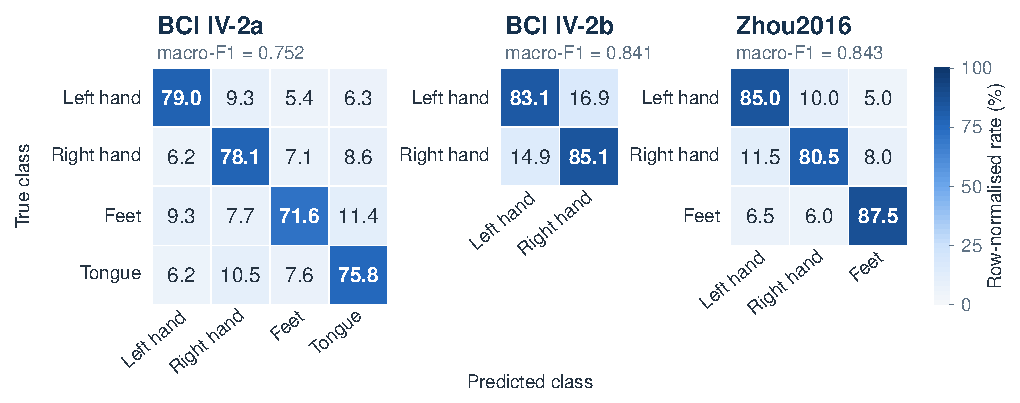
\includegraphics[width=0.92\textwidth]{figures/classwise_confusion.pdf}
\caption{Ma trận nhầm lẫn trung bình của SSM-DAN trên các phiên đánh giá của BCI IV-2a (trái), BCI IV-2b (giữa) và Zhou2016 (phải). Ma trận của mỗi chủ thể được chuẩn hóa theo số lần thử của từng lớp thật rồi lấy trung bình trên các chủ thể đích, nên đường chéo cho độ nhạy trung bình của mỗi lớp; điểm F1 trung bình macro được ghi dưới tên mỗi bộ dữ liệu.}
\label{fig:classwise}
\end{figure*}

Hình~\ref{fig:classwise} cho thấy các mức tăng này trải đều trên các lớp chứ không đạt được bằng cách ưu tiên một lớp dễ: macro-F1 bám sát độ chính xác trên mọi bộ dữ liệu và không lớp nào bị bỏ qua một cách có hệ thống. Điều này quan trọng với thích ứng tại thời điểm kiểm thử, vì hàm mục tiêu entropy có thể khiến dự đoán sụp về một vài lớp. Các lỗi còn lại cũng hợp lý về mặt sinh lý: trên BCI IV-2a, tưởng tượng chân bị nhầm nhiều nhất với tưởng tượng lưỡi, hai tác vụ được biểu diễn gần đường giữa của vỏ não cảm giác--vận động, trong khi các lớp tay lệch bên được nhận dạng tốt nhất.

\subsection{So sánh với các kết quả đã công bố}
\label{subsec:published}

Bảng~\ref{tab:published} đối chiếu độ chính xác liên chủ thể được báo cáo trong các bài báo gốc với kết quả chạy lại trong nghiên cứu này. Các giá trị đã công bố không so sánh trực tiếp được, vì các giao thức khác nhau ở bốn điểm. (i) \emph{Tác vụ}: các bài T-TIME và BFT báo cáo MI hai lớp tay trái so với tay phải, trong khi BCI IV-2a và Zhou2016 ở đây được đánh giá với bốn và ba lớp. (ii) \emph{Dịch chuyển phiên và dữ liệu đích}: một số giao thức huấn luyện và kiểm thử trong cùng một phiên ghi, và bài EEGEncoder hoàn toàn không báo cáo kết quả liên chủ thể, con số đa chủ thể của họ thu được khi tập huấn luyện chứa cả phiên đầu của chính các chủ thể kiểm thử; ở đây mọi chủ thể đích đều chưa được thấy khi huấn luyện và được chấm điểm trên một phiên sau, ghi vào ngày khác. (iii) \emph{Chọn mô hình}: các script công bố của SATrans-Net và RMETNet báo cáo độ chính xác theo epoch cao nhất, hoặc trung bình năm giá trị cao nhất, trên chủ thể bị giữ lại, tức nhãn đánh giá được dùng để chọn epoch; ở đây checkpoint chỉ được chọn dựa trên dữ liệu nguồn. (iv) \emph{Truy cập chuyển nạp (transductive)}: RMETNet dùng chính các lần thử đánh giá bị giữ lại làm miền đích cho hàm MMD và căn chỉnh Riemann, trong khi ở đây thích ứng miền chỉ thấy các phiên đích trước đó, không nhãn. Mỗi điểm (ii)--(iv) làm giao thức dễ hơn hoặc ước lượng lạc quan hơn, điều này phần lớn giải thích vì sao hầu hết kết quả chạy lại thấp hơn trên BCI IV-2a. Khi cách chia khớp với của chúng tôi, chênh lệch nhỏ: benchmark của TCFormer \cite{altaheri2025tcformer} dùng cùng cách chia phiên và chỉ khác ở việc lấy trung bình mô hình epoch cuối trên năm hạt giống và tiền xử lý riêng theo mô hình, và kết quả chạy lại của TCFormer và ATCNet nằm trong phạm vi ba điểm so với benchmark đó trên cả hai bộ BCI, còn EEG Conformer ở đây cao hơn. Trên BCI IV-2b, nơi dịch chuyển giữa phiên hiệu chuẩn và phiên đánh giá nhỏ hơn, kết quả chạy lại đạt hoặc vượt một số giá trị đã công bố (ví dụ SATrans-Net, 81,76 so với 79,64\%).

\begin{table*}[!htbp]
\centering
\caption{Độ chính xác liên chủ thể (\%) đã công bố của các phương pháp cơ sở so với kết quả chạy lại theo giao thức của nghiên cứu này (Bảng~\ref{tab:protocol}). --: không báo cáo; các thiết lập (a)--(e) được nêu dưới bảng.}
\label{tab:published}
\footnotesize
\setlength{\tabcolsep}{4pt}
\begin{adjustbox}{max width=\textwidth}
\begin{tabular}{llccc@{\hspace{14pt}}ccc}
\toprule
 & & \multicolumn{3}{c}{Đã công bố} & \multicolumn{3}{c}{Nghiên cứu này (LOSO theo thời gian)} \\
\cmidrule(lr){3-5}\cmidrule(lr){6-8}
Phương pháp & Thiết lập & BCI IV-2a & BCI IV-2b & Zhou2016 & BCI IV-2a & BCI IV-2b & Zhou2016 \\
\midrule
EEG Conformer~\cite{song2023eegconformer} & (a)~\cite{altaheri2025tcformer} & 45.59 & 75.25 & -- & 55.25 & 78.03 & 77.17 \\
ATCNet~\cite{altaheri2023atcnet} & (a)~\cite{altaheri2025tcformer} & 59.66 & 80.94 & -- & 57.02 & 79.38 & 76.50 \\
TCFormer~\cite{altaheri2025tcformer} & (a) & 63.00 & 81.34 & -- & 60.80 & 81.18 & 73.50 \\
EEGEncoder~\cite{liao2025eegencoder} & (b) & -- & -- & -- & 58.06 & 81.02 & 74.33 \\
SATrans-Net~\cite{miao2025satransnet} & (c) & 68.13 & 79.64 & -- & 62.00 & 81.76 & 74.67 \\
RMETNet~\cite{zhao2026rmetnet} & (d) & 71.39 & 80.93 & -- & 60.11 & 79.10 & 81.17 \\
T-TIME~\cite{li2024ttime} & (e) & 79.30$^{\dagger}$ & -- & -- & 66.24 & 79.03 & 85.00 \\
BFT~\cite{li2026bft} & (e) & 77.47$^{\dagger}$ & -- & 84.38$^{\dagger}$ & 63.08 & 81.18 & 82.83 \\
\bottomrule
\end{tabular}
\end{adjustbox}
\par\smallskip
\begin{minipage}{\textwidth}\scriptsize
(a) Cùng cách chia phiên như ở đây, mô hình epoch cuối lấy trung bình trên năm hạt giống, tiền xử lý riêng theo mô hình. (b) Không có kết quả liên chủ thể; con số 74,48\% trên BCI IV-2a huấn luyện trên phiên~1 của mọi chủ thể, kể cả chủ thể kiểm thử. (c) LOSO không nêu cách chia phiên, lấy độ chính xác kiểm thử cao nhất theo epoch. (d) Một phiên cho mỗi chủ thể, chủ thể bị giữ lại được dùng làm đích cho MMD/RA, trung bình năm epoch tốt nhất. (e) Thích ứng tại thời điểm kiểm thử trực tuyến chỉ trên phiên~1. $^{\dagger}$Tác vụ hai lớp (tay trái so với tay phải).
\end{minipage}
\end{table*}

\subsection{Nghiên cứu loại bỏ thành phần}
\label{sec:ablation}

Bảng~\ref{tab:ablation} tuân theo giao thức chính theo thời gian. Biến thể không có thích ứng miền loại bỏ mọi thành phần thích ứng miền ở Giai đoạn~1 (AutoDIAL, cực đại hóa thông tin trên đích, hàm mất mát đối kháng và cả hai hàm MMD) nhưng giữ lại căn chỉnh Riemann và IM-TTA; ngoài ra, mọi biến thể dùng cùng các lượt và cùng quy tắc chọn checkpoint.

\begin{table*}[!htbp]
\centering
\caption{Kết quả loại bỏ thành phần: trung bình $\pm$ độ lệch chuẩn của độ chính xác (\%) và $\kappa$ của Cohen trên các chủ thể đích.}
\label{tab:ablation}
\small
\setlength{\tabcolsep}{3.0pt}
\begin{tabular}{llcccc}
\toprule
Bộ dữ liệu & Thước đo & SSM-DAN & \colhead{Không có\\căn chỉnh\\Riemann} & \colhead{Không có\\thích ứng\\miền} & \colhead{Không có\\thích ứng tại\\thời điểm kiểm thử} \\
\midrule
\multirow{2}{*}{BCI IV-2a}
 & Đ.c.x. & $\mathbf{76.12\pm11.96}$ & $70.29\pm11.60$ & $71.37\pm11.78$ & $72.15\pm13.58$ \\
 & $\kappa$ & $\mathbf{0.682\pm0.159}$ & $0.604\pm0.155$ & $0.618\pm0.157$ & $0.629\pm0.181$ \\
\midrule
\multirow{2}{*}{BCI IV-2b}
 & Đ.c.x. & $\mathbf{84.09\pm10.42}$ & $83.58\pm10.46$ & $83.35\pm10.50$ & $83.97\pm10.71$ \\
 & $\kappa$ & $\mathbf{0.682\pm0.208}$ & $0.672\pm0.209$ & $0.667\pm0.210$ & $0.679\pm0.214$ \\
\midrule
\multirow{2}{*}{Zhou2016}
 & Đ.c.x. & $\mathbf{84.33\pm0.75}$ & $84.00\pm3.16$ & $82.50\pm1.85$ & $82.33\pm3.82$ \\
 & $\kappa$ & $\mathbf{0.765\pm0.011}$ & $0.760\pm0.047$ & $0.738\pm0.028$ & $0.735\pm0.057$ \\
\bottomrule
\end{tabular}
\end{table*}

Trên BCI IV-2a, việc loại bỏ căn chỉnh Riemann, thích ứng miền Giai đoạn~1, hoặc thích ứng tại thời điểm kiểm thử đều làm giảm độ chính xác có ý nghĩa thống kê. Trên BCI IV-2b và Zhou2016, mô hình đầy đủ vẫn là biến thể tốt nhất, nhưng mức chênh nhỏ và không có ý nghĩa. Do đó, đóng góp của từng thành phần phụ thuộc vào bộ dữ liệu.

\subsection{Vì sao căn chỉnh Riemann giúp ích trên BCI IV-2a}
\label{subsec:ra_mechanism}

Phân tích chẩn đoán hình học phân biệt việc co các miền lại gần nhau nói chung với kiểu căn chỉnh thực sự hữu ích cho phân loại (Hình~\ref{fig:ra_label_selectivity}). Trên các tác vụ gốc, độ chính xác theo tâm gần nhất tăng từ 30,32\% lên 42,52\% trên BCI IV-2a ($+12,19$ điểm phần trăm; Wilcoxon theo cặp chính xác $p=0,0039$), nhưng chỉ từ 56,66\% lên 57,63\% trên BCI IV-2b ($+0,97$ điểm; $p=0,4961$). Quan trọng hơn, mức tăng biên quyết định chuẩn hóa là 0,1517 trên BCI IV-2a bốn lớp so với 0,0287 trên BCI IV-2b hai lớp (kiểm định hoán vị chính xác $p_\mathrm{Holm}=0,0389$). Hiệu ứng vẫn còn khi BCI IV-2a được rút xuống C3/Cz/C4 (0,2264; $p_\mathrm{Holm}=0,0110$ so với BCI IV-2b), loại trừ khả năng số kênh là nguyên nhân duy nhất.

\begin{figure*}[!htbp]
\centering
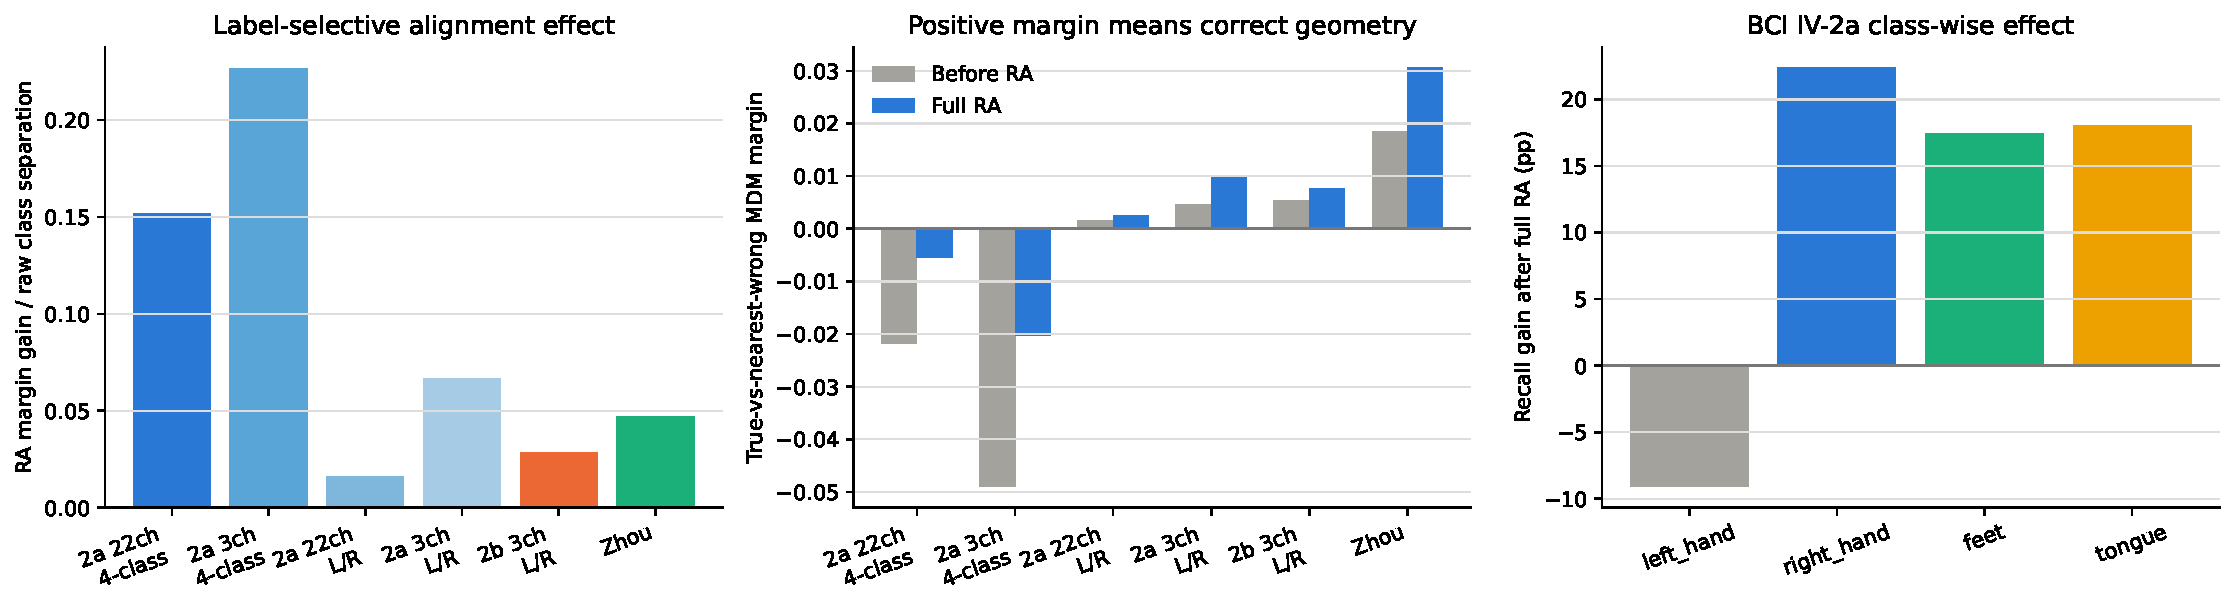
\includegraphics[width=\textwidth]{../../../../analysis/ra_mechanism_outputs/ra_label_selectivity.pdf}
\caption{Hiệu ứng chọn lọc theo nhãn của RA. Trái: mức tăng theo từng chủ thể của biên Riemann giữa lớp đúng và lớp sai gần nhất (Pt.~\ref{eq:mdm_margin}), chuẩn hóa bằng độ tách biệt giữa các lớp nguồn trước RA; hình thoi và thanh biểu thị trung bình và khoảng tin cậy bootstrap 95\%. Giữa: biên thô trung bình trước và sau RA đầy đủ, giá trị dương biểu thị hình học lớp đúng. Phải: thay đổi theo lớp của độ nhạy MDM chẩn đoán trên tác vụ BCI IV-2a 22 kênh gốc. Phân tích chẩn đoán không dùng mô hình này tách biệt với độ chính xác của SSM-DAN.}
\label{fig:ra_label_selectivity}
\end{figure*}

Trong BCI IV-2a, giới hạn tác vụ về trái/phải làm mức tăng biên chuẩn hóa giảm từ 0,1517 xuống 0,0160 với 22 kênh ($p_\mathrm{Holm}=0,0389$) và từ 0,2264 xuống 0,0665 với ba kênh ($p_\mathrm{Holm}=0,0234$). RA đầy đủ đặc biệt phục hồi các lớp có khả năng chuyển giao kém khi chưa căn chỉnh: độ nhạy chẩn đoán tăng lần lượt 22,38, 17,44 và 18,06 điểm cho tay phải, chân và lưỡi, trong khi độ nhạy tay trái giảm 9,10 điểm. Ngược lại, khi khớp cả cấu hình ba kênh lẫn tác vụ trái/phải, khác biệt về mức tăng biên giữa BCI IV-2a và IV-2b không có ý nghĩa ($p=0,4174$). Như vậy, bằng chứng chỉ về phía hình học hiệp phương sai có điều kiện theo lớp phong phú hơn của tác vụ bốn lớp gốc trên BCI IV-2a, chứ không phải chỉ số điện cực hay độ lớn của dịch chuyển biên. Phân tích chẩn đoán này giải thích chiều hướng của phép loại bỏ trên mạng nơ-ron nhưng bản thân nó không phải là kết quả độ chính xác của SSM-DAN.

\subsection{Hiệu năng tính toán}
\label{subsec:results_efficiency}

Bảng~\ref{tab:efficiency} báo cáo số tham số huấn luyện được, thời gian huấn luyện Giai đoạn~1 và thời gian phản hồi trên CPU. Biến thể chỉ dùng nguồn nhỏ hơn vì không có lớp AutoDIAL, bộ căn chỉnh và bộ phân biệt miền; RA và IM-TTA không làm thay đổi số tham số.

Thích ứng Giai đoạn~1 chiếm phần lớn thời gian huấn luyện tăng thêm của SSM-DAN so với biến thể chỉ dùng nguồn (gần gấp đôi trên Zhou2016), trong khi IM-TTA chỉ thêm rất ít. SSM-DAN có số tham số tương đương ATCNet và TCFormer, thấp hơn nhiều so với EEG Conformer, còn T-TIME và BFT là các phương pháp nhỏ và nhanh nhất.

\begin{table*}[!htbp]
\centering
\caption{Chi phí tính toán: số tham số huấn luyện được, thời gian huấn luyện Giai đoạn~1 trung bình mỗi lượt, và thời gian phản hồi CPU cho một lần thử. Các biến thể SSM-DAN như ở Mục~\ref{subsec:baselines}.}
\label{tab:efficiency}
\small
\setlength{\tabcolsep}{2pt}
\begin{adjustbox}{max width=\textwidth}
\begin{tabular}{>{\raggedright\arraybackslash}p{2.75cm}@{\hspace{2pt}}ccc@{\hspace{2pt}}ccc@{\hspace{2pt}}ccc}
\toprule
 & \multicolumn{3}{c}{BCI IV-2a} & \multicolumn{3}{c}{BCI IV-2b} & \multicolumn{3}{c}{Zhou2016} \\
\cmidrule(lr){2-4}\cmidrule(lr){5-7}\cmidrule(lr){8-10}
Phương pháp & Tham số & Huấn luyện & CPU & Tham số & Huấn luyện & CPU & Tham số & Huấn luyện & CPU \\
 & (K) & (phút) & (ms) & (K) & (phút) & (ms) & (K) & (phút) & (ms) \\
\midrule
\multicolumn{10}{l}{\textit{Huấn luyện chỉ dùng nguồn}} \\
Conformer & 789.6 & 11.14 & 11.45 & 759.1 & 4.93 & 9.34 & 858.7 & 1.53 & 10.34 \\
ATCNet & 113.7 & 48.58 & 13.33 & 112.8 & 60.19 & 11.35 & 113.3 & 8.09 & 11.91 \\
TCFormer & 127.2 & 38.37 & 14.96 & 123.4 & 31.04 & 11.17 & 125.6 & 5.89 & 15.97 \\
EEGEncoder & 197.2 & 13.49 & 26.51 & 196.2 & 14.98 & 26.88 & 196.8 & 3.64 & 25.68 \\
SATrans-Net & 155.6 & 10.19 & 12.78 & 153.7 & 4.99 & 11.10 & 155.0 & 1.32 & 11.38 \\
SSM-DAN (chỉ nguồn) & 98.4 & 47.01 & 25.08 & 94.6 & 36.10 & 13.68 & 96.8 & 6.29 & 13.36 \\
\midrule
\multicolumn{10}{l}{\textit{Thích ứng miền không giám sát}} \\
RMETNet & 193.8 & 45.88 & 11.15 & 159.1 & 21.96 & 4.90 & 306.6 & 23.74 & 7.19 \\
SSM-DAN (UDA Giai đoạn~1) & 132.0 & 58.45 & 18.44 & 128.2 & 48.08 & 13.35 & 130.4 & 11.42 & 14.65 \\
\midrule
\multicolumn{10}{l}{\textit{Thích ứng tại thời điểm kiểm thử}} \\
T-TIME & 9.5 & 5.85 & 7.71 & 6.3 & 3.07 & 5.08 & 8.4 & 1.34 & 6.72 \\
BFT & 40.6 & 1.47 & 3.08 & 39.9 & 0.96 & 2.61 & 51.0 & 0.36 & 2.84 \\
SSM-DAN (IM-TTA) & 131.9 & 40.73 & 22.12 & 128.1 & 33.21 & 14.25 & 130.3 & 6.46 & 18.41 \\
\midrule
SSM-DAN\newline (không RA) & 132.0 & 58.41 & 21.63 & 128.2 & 47.95 & 13.33 & 130.4 & 11.66 & 18.88 \\
\textbf{SSM-DAN} & \textbf{132.0} & \textbf{59.82} & \textbf{22.20} & \textbf{128.2} & \textbf{54.21} & \textbf{17.40} & \textbf{130.4} & \textbf{11.70} & \textbf{19.14} \\
\bottomrule
\end{tabular}
\end{adjustbox}
\end{table*}

\section{Thảo luận}
\label{sec:discussion}

Lợi ích của từng thành phần thích ứng phụ thuộc vào bộ dữ liệu: rõ rệt trên BCI IV-2a nhưng nhỏ và không có ý nghĩa trên BCI IV-2b và Zhou2016, nơi cần các thí nghiệm lặp với nhiều hạt giống để xác nhận khác biệt. Phân tích hình học gợi ý rằng sự khác biệt này được quyết định bởi tính chọn lọc theo nhãn chứ không phải mức độ RA co các miền lại gần nhau: RA đầy đủ làm giảm dịch chuyển hiệp phương sai có điều kiện theo lớp trên BCI IV-2b, nhưng hầu như không cải thiện biên giữa lớp đúng và lớp sai. Trên BCI IV-2a, hiệu ứng vẫn tồn tại khi rút xuống ba kênh nhưng yếu đi đáng kể khi tác vụ bốn lớp được rút về trái/phải. Vì vậy, RA có vẻ đặc biệt hữu ích cho các mẫu hiệp phương sai lệch bên và đường giữa không đồng nhất của tác vụ này; kết quả không hàm ý rằng tăng số lớp nói chung sẽ cải thiện RA.

Các lượt quét xen kẽ khai thác trọn vẹn các lần thử ngoại tuyến và không nhân quả, nên ứng dụng trực tuyến sẽ cần xử lý chỉ theo chiều xuôi.

Do IM-TTA sử dụng tín hiệu không nhãn của phiên đánh giá, phương pháp mang tính chuyển nạp và phải được so sánh với các phương pháp cơ sở có cùng mức truy cập dữ liệu đích. Các hạn chế khác gồm thiết lập ba kênh của BCI IV-2b, số người tham gia ít của Zhou2016, và các phương pháp cơ sở tương ứng chưa đầy đủ.

\section{Kết luận}
\label{sec:conclusion}

Chúng tôi đã trình bày SSM-DAN, một khung MI-EEG liên chủ thể kết hợp tích chập đa thang và mô hình không gian trạng thái chọn lọc hai chiều với UDA phân cấp và IM-TTA có ràng buộc, được đánh giá theo giao thức LOSO theo thời gian, giữ nhãn đích nằm ngoài huấn luyện, thích ứng và chọn mô hình. Phương pháp đạt độ chính xác trung bình 76,12\% trên BCI IV-2a, 84,09\% trên BCI IV-2b và 84,33\% trên Zhou2016. Vẫn cần các phương pháp cơ sở tương ứng và thí nghiệm lặp với nhiều hạt giống trước khi rút ra kết luận rộng hơn.

\section*{Đóng góp của tác giả theo CRediT}
\textbf{[Tên tác giả]:} Lên ý tưởng, Phương pháp luận, Phần mềm, Kiểm chứng, Phân tích hình thức, Điều tra, Quản lý dữ liệu, Trực quan hóa, Viết -- bản thảo đầu, Viết -- rà soát và chỉnh sửa.

\section*{Tuyên bố xung đột lợi ích}
Các tác giả tuyên bố không có xung đột lợi ích tài chính hay quan hệ cá nhân nào có thể ảnh hưởng đến công trình được báo cáo trong bài báo này.

\section*{Tài trợ}
Nghiên cứu này không nhận tài trợ cụ thể nào từ các cơ quan tài trợ thuộc khu vực công, thương mại hay phi lợi nhuận.

\section*{Tính sẵn có của dữ liệu}
Toàn bộ dữ liệu EEG được phân tích trong nghiên cứu này đều công khai. Các bộ dữ liệu BCI Competition IV 2a và 2b \cite{tangermann2012review} và bộ dữ liệu Zhou2016 \cite{zhou2016trialselection} được truy cập qua thư viện MOABB \cite{jayaram2018moabb}; không thu thập dữ liệu mới.

\bibliographystyle{elsarticle-num}
\bibliography{references}

\end{document}

\endinput
